\documentclass[11pt,a4paper]{article}
\usepackage[margin=3cm]{geometry}
\usepackage[english]{babel}
\usepackage[dvipsnames]{xcolor}
\usepackage[utf8x]{inputenc}
\usepackage{amsmath}
\usepackage{graphicx}
\setlength {\marginparwidth }{2cm}
\usepackage[colorinlistoftodos]{todonotes}
\usepackage{setspace}
\usepackage{etoolbox}
\usepackage{framed,color}
\usepackage{tcolorbox}
\usepackage[english]{babel}
\usepackage[nottoc]{tocbibind}
\usepackage{float}
\usepackage{pdfpages}
\renewcommand{\baselinestretch}{1.3}

\begin{document}

\begin{titlepage}

\newcommand{\HRule}{\rule{\linewidth}{0.5mm}} % Defines a new command for the horizontal lines, change thickness here

\center % Center everything on the page

%----------------------------------------------------------------------------------------
%	HEADING SECTIONS
%----------------------------------------------------------------------------------------

\textsc{\LARGE New Zealand}\\[0.5cm]

\textsc{\LARGE  Maritime School}\\[1.5cm]
\textsc{\Large ETO Course 942.469}\\[0.2cm] % Major heading such as course name
\textsc{\large Electrical and Electronic Measuring Equipment, Basic Electrical Fault Finding}\\[0.5cm] % Minor heading such as course title

%----------------------------------------------------------------------------------------light
%	TITLE SECTION
%----------------------------------------------------------------------------------------

\HRule \\[0.5cm]
{ \huge \bfseries Module Assignment}\\[0.2cm] % Title of your document
\HRule \\[0.5cm]
\begin{minipage}{0.4\textwidth}
\begin{flushleft} \large
\emph{Author:}\\
Levi \textsc{Dubbelman}

\textit{SN: 190000929}\par
\end{flushleft}
\end{minipage}
~
\begin{minipage}{0.4\textwidth}
\begin{flushright} \large
\emph{Supervisors:} \\
John \textsc{Lamb} \&

Nick \textsc{Cossar}
\end{flushright}
\end{minipage}\\[2cm]
{\large May, 2019}\\[2cm]

\includegraphics[width=4cm]{logo.png}
\vfill
\end{titlepage}
\tableofcontents
\newpage
% BEGINNING OF LEARNING OUTCOME 1
\section*{Learning Outcome 1}
\begin{tcolorbox}[colback=red!5!white,colframe=red!75!black,title=\textbf{Demonstrate basic knowledge of the implementation of satisfactory safety procedures}]
Research into these topics and produce a structured assignment ( including references to web sites and photos/schematics ) to demonstrate your basic understanding of the construction and operational characteristics of the following:-
\begin{itemize}
\item Shipboard LV and HV AC – generating – distribution and propulsion systems
\item Ships onboard DC grid – hybrid AC/DC - generating – distribution and propulsion systems
\item Your thoughts on future technologies for shipboard electrical - generating – distribution and propulsion systems
\item Examine a small selection of typical shipboard electrical equipment (eg – two engine room machines or equipment) to show a basic understanding of construction and operation characteristics.
\end{itemize}
\end{tcolorbox}
\section{Low Voltage AC}
Ships with low electrical power demands may use a low voltage system. This system is typically three-phase 440V or 690V at 60 Hz (AC). This system is usually an unearthed, insulated system for earth fault redundancy.
\subsection*{Generation}
Low voltage will be generated by onboard diesel engines driving a synchronous AC alternator. Occasionally, a shaft generator or turbo-alternator system may be used, however their unstable frequencies generally prevent parallel operation with the diesel generators. In addition, a separate switchboard containing essential consumers necessary for safe of life at sea will have their own emergency diesel generator. This emergency generator will typically be of different construction and operating characteristics as the primary generation. This prevents parallel operation. The Maersk line EEE ships also use an economizer boiler and shaft generator which can also act as a motor, allowing for greater fuel efficiency when the engines are at Full Ahead.
\subsection*{Distribution}
Ships using low voltage at 440V or 690V will also have low voltage transformers for 240V consumers. They may also have battery banks or panel LEDs with a rectifier arrangement. The primary switchboard and bus bar array will be located within the engine control room, as there is low risk of an arc explosion at these voltages. Their circuit breakers are typically Moulded Case Circuit Breakers (MCCB) with either air separation or sulfur-hexaflouride separation. Vacuum circuit breakers are generally unnecessary.
\subsection*{Propulsion}
Low voltage ships generally do not use electric for primary propulsion. Rather, their prime mover will be a two-stroke engine with exceptional bore and stroke length characteristics. This engine may drive a shaft generator. In addition, recent advancements in technology allow modern two-stroke engines to do away with their camshaft driving rocker arms and a poppet valve arrangement to instead use either an electromagnetic, hydraulic or pneumatic to open and close the poppet valves. This allows for higher degrees of fuel efficiency. These ships will typically still use one or more bow or stern thrusters which are electrically driven. However, they may start with either a variable frequency drive or a star-delta configuration to reduce starting current, which would otherwise tax the diesel generators too harshly.
\section{High Voltage AC}
Ships with high electrical power demands may use a high voltage system. This system is typically three-phase 3.3kV, 6.6kV or 11kV at 60 Hz (AC). This system is usually earthed by a resistor, known as a Neutral Earth Resistor (NER). Earthing down ensures all the stored electrical energy in the circuit insulation is safely discharged to earth.
\subsection*{Generation}
High voltage is typically generated by onboard diesel or dual-fuel engines driving a synchronous AC alternator. Occasionally, a steam or gas turbine will be used instead. This has the advantage of lower emissions, but requires very light fuel, which is expensive. As with low voltage ships, an emergency generator and switchboard will be used. This generator is typically low voltage.
\subsection*{Distribution}
Ships using high voltage will have separate switchboards for high voltage and low voltage. High voltage switchboards require additional safety precautions to prevent arc events. These will typically use vacuum or sulfur-hexaflouride circuit breakers. Air circuit breakers do not provide enough arc dispersion effect to be used safely at sea, despite their frequent use on land. In addition to transformers used for low voltage consumers, ships using high voltage will also typically also use electric propulsion, which require drive transformers, usually at 1800-2200 Volts.
\subsection*{Propulsion}
Propulsion Electric Motors, or PEMs, are the most common form of propulsion on high voltage ships. These may be a thruster arrangement, e.g. Azimuth thrusters, or Z-drive thrusters, or they may be a screw arrangement. It is common for both types to use a half-motor whereby the windings are interlaced between each other, allowing for greater redundancy and speed control. Recent advancements in electric motor designs include the Advanced Induction Motor, using a DC bridge rectifier/inverter system to produce four or more phases in an induction motor. This is especially useful for warships where shock is a factor, as the AIM has a large air gap between stator and rotor.
\begin{center}
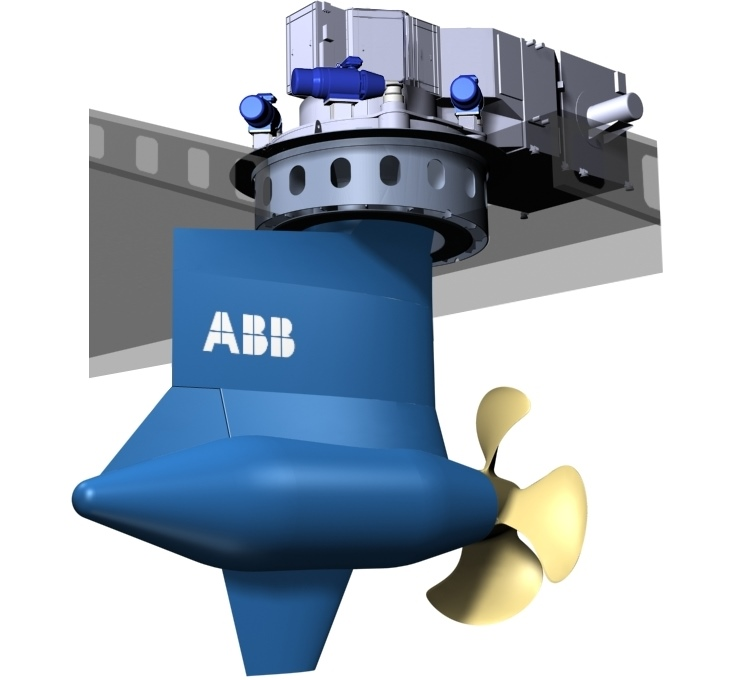
\includegraphics[width=6cm]{azi}
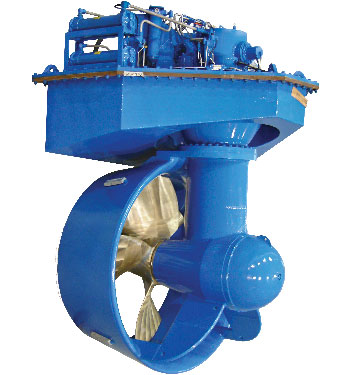
\includegraphics[width=6cm]{zi}

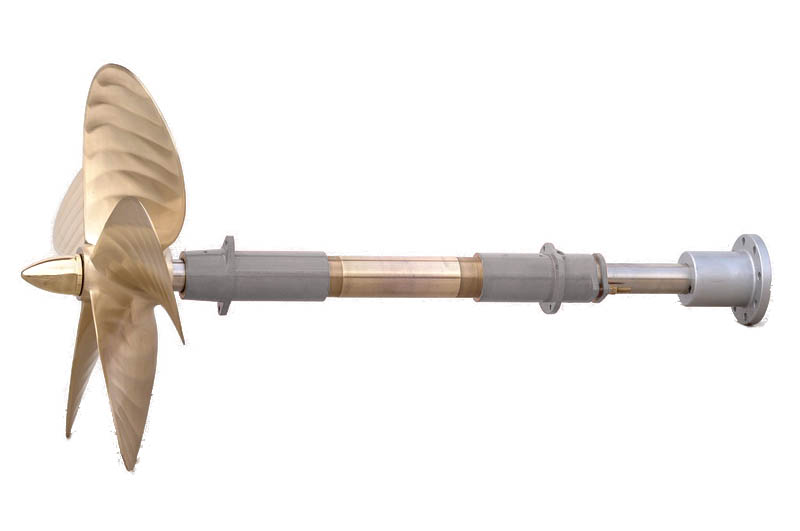
\includegraphics[width=10cm]{pem}\par
An Azipod, a Z-Drive thruster and a shaft/prop arrangement.
\end{center}
\section{Onboard DC Grid}
Very recent advancements in DC power electronics allow the onboard DC grid to be used in ships. This system has been spearheaded by ABB, and includes advantages over traditional AC grids, such as variable speed generators for fuel efficiency, increased "useful" capacity, e.g. cargo space, due to an absence of transformers.
\subsection*{Generation}
DC Grid generators will typically still be AC synchronous machines, with one important difference. The AC generated will be immediately rectified to DC. This essentially means there is no requirement for a fixed speed generator, which otherwise would have frequency indexed to RPM.
\subsection*{Distribution}
DC distribution is significantly different to AC distribution. The most striking example of this is the inability to break DC current flow using conventional circuit breakers. Rather than simply discharging until the zero point, like on AC, the DC must be electronically switched off before breaking the circuit. Another advantage of DC is the safety against electrocution. In AC, there will always be present a capacitive earthing, which allows electrocution to occur at phase voltage -- which is often deadly. However, in a DC system, a pathway from positive to negative needs to exist -- meaning electrocution can only occur when touching both positive and negative -- or if an earth fault exists.
\subsection*{Propulsion}
Propulsion on DC is similar to propulsion on high voltage AC, with an important difference. Variable Frequency Drives have one less layer of complexity -- no rectifier/DC bridge. This allows for simplified inverter drives which require no DC bridge. Alternatively, brushless DC motors may be used, such as the Rolls Royce Mermaid's permanent magnet range of azimuth thrusters.
\begin{center}
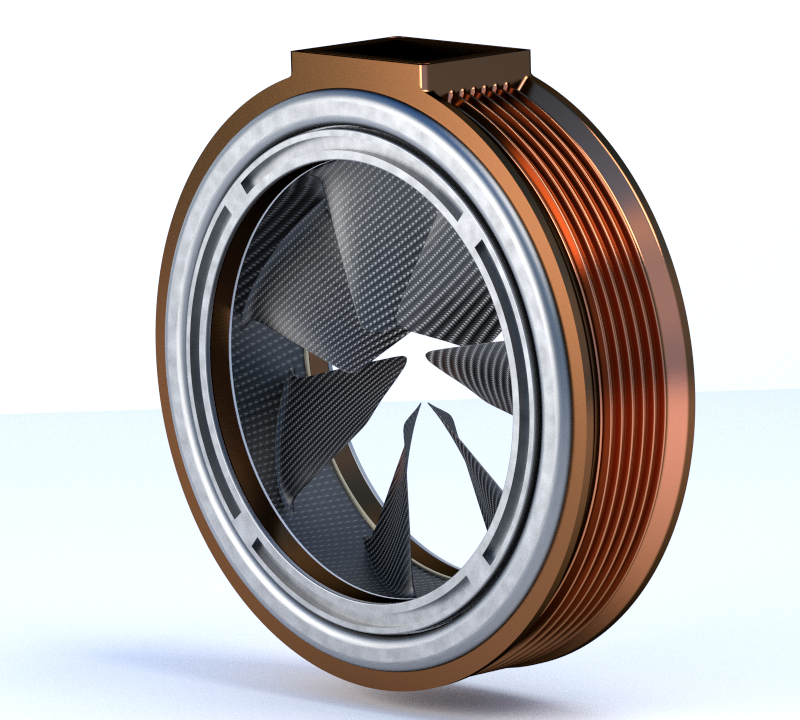
\includegraphics[width=6cm]{rdp}\par
A Rim Driven Propeller (RDP), a new form of BLDC propulsion.
\end{center}
\section{Hybrid AC/DC Grid}
Providing the best of both worlds, some ships may opt to use a hybrid AC/DC system with two independent distribution grids. This unfortunately does not eliminate the need of large transformers, or allow the diesel generators to operate at variable speeds, however it allows the ship to more easily invert DC to AC for AC consumers who would benefit from variable speed control.
\subsection*{Generation}
Power is still generated in AC as it would with a simply AC ship, and distributed to fixed frequency AC consumers. However, any additional DC sources such as solar arrays can be connected seamlessly to the DC side of the grid.
\subsection*{Distribution}
Instead of a main switchboard simply distributing AC to fixed frequency AC consumers, the AC is instead rectified to DC for a separate DC grid -- allowing more effective speed control with less componentry for AC consumers. In addition, the DC is used for battery arrays.
\subsection*{Propulsion}
The benefits of a Hybrid AC/DC system is most noticeable in propulsion. By removing the rectifier-inverter components and instead simply inverting the DC, it provides greater efficiency and less componentry for variable speed control for propulsion electric motors.
\section{Future Technologies}
The future of Maritime is extremely exciting. I predict a focus on taking existing technologies and focusing on improving its efficiency. The philosophy in the Maritime industry is one of clean, efficient, safe and effective. To this end, I expect A.I. (Artificial Intelligence) or V.I. (Virtual Intelligence) assistance for nautical and technical crew. What I mean is, either Augmented Reality tools or holographic projections on bridge, or in the E.C.R. as an ever-growing increase in technical information is recorded and displayed to crew, to the point where potentiometer-based instrumentation is simply too bulky and ineffective at displaying variable information.
\begin{center}
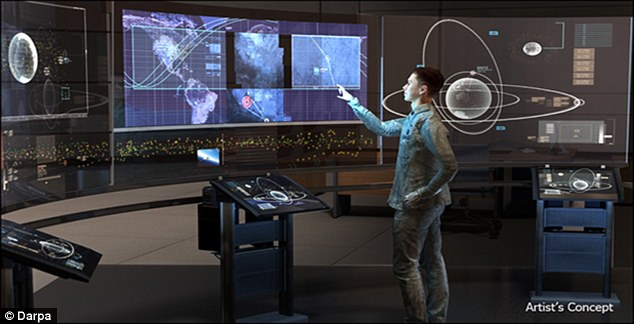
\includegraphics[width=10cm]{controlcenter}\par
A concept command center
\end{center}
\subsection*{Generation}
I believe that LNG/MDO mixtures will become more common. I also foresee battery-only with diesel emergency generators being used more frequently in passenger or roll-on roll-off ferries or ships with very predictable, oft-repeated routes such as riverway cargo. I expect an increase in hydrogen fuel cells -- potentially using resonant frequency to separate hydrogen from water. I expect wave generation technology to be used in certain ships, as well as wind power. Barring any revolutions in battery technology, I also foresee a potential move to kinetic energy storage methods, similar to the TERALOOP project out of France.

\begin{center}
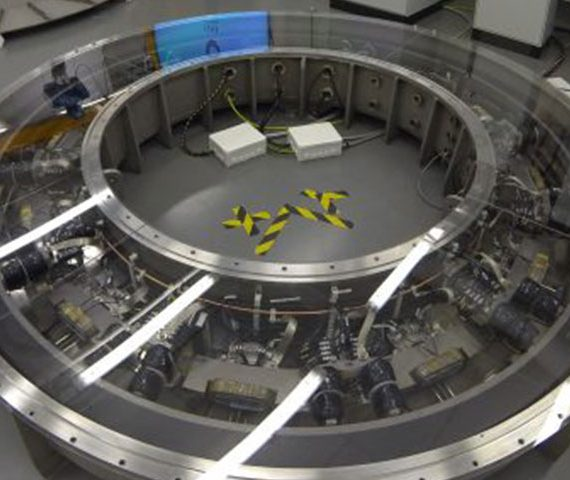
\includegraphics[width=8cm]{teraloop}\par
The TERALOOP kinetic disk energy storage and transfer system
\end{center}
\subsection*{Distribution}
Due to the inherent nature of DC where power factor is non existent, and the only impedance is resistive, I believe that there will be a greater increase in ships with an Onboard DC Grid. I believe that there will be a greater increase in renewable DC power -- such as efficient solar, wind or battery power sources -- being used, especially on coastal ships.
\subsection*{Propulsion}
I believe there will be a increase in brushless DC motors or rim-driven thrusters being used on ship of increasing size as permanent magnet technology improves. I also foresee a potential return to sails being used as propulsion for cruise ships -- however, I do not believe sails will be used on cargo or offshore ships as it is an unpredictable method of propulsion.
\begin{center}
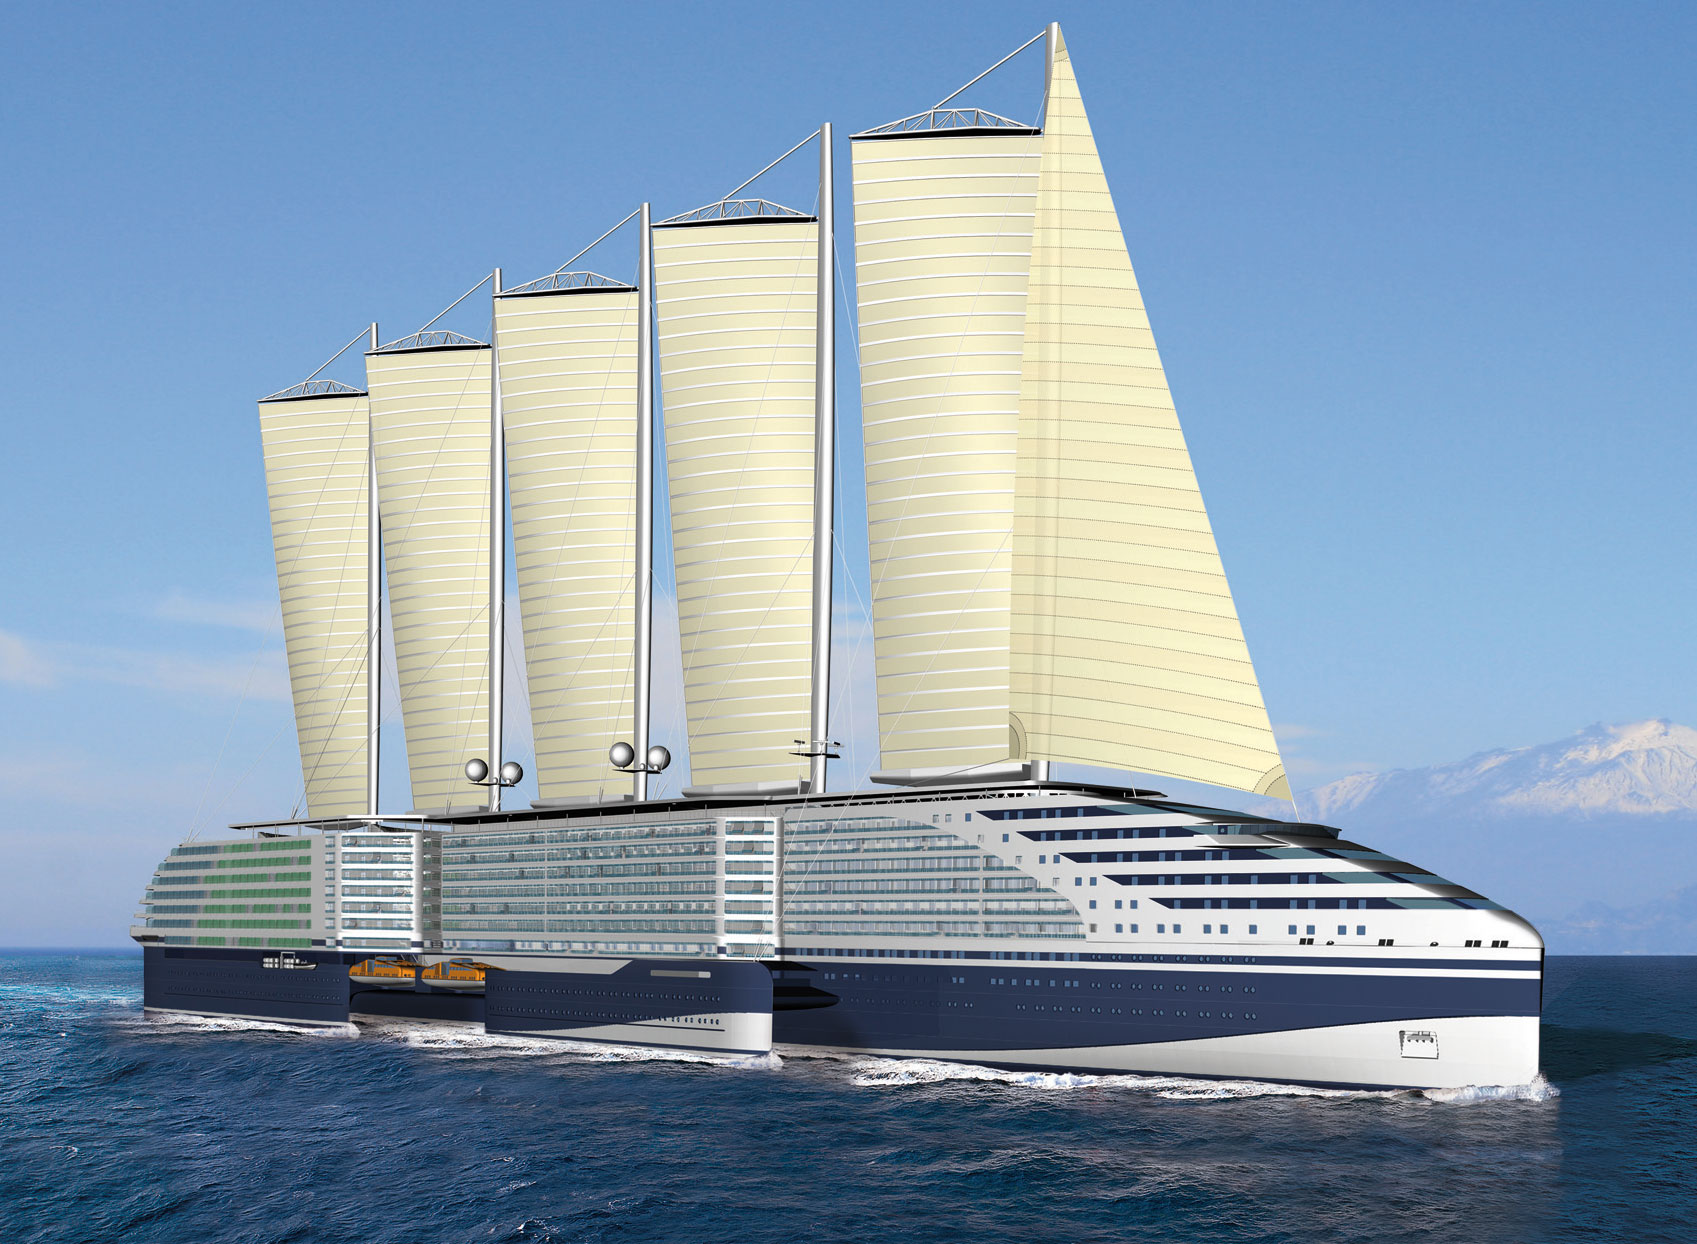
\includegraphics[width=10cm]{stx}\par
The \textit{STX Eoseas} -- a concept cruise ship with sails and a pentamaran hull.
\end{center}
\section{Programmable Logic Controllers}
Programmable Logic Controllers, or PLCs, are small, simple, rugged computers found commonly in automation systems. Common PLC brands include Allan-Bradley, Siemens, Schneider-Electric and ABB.
\begin{center}
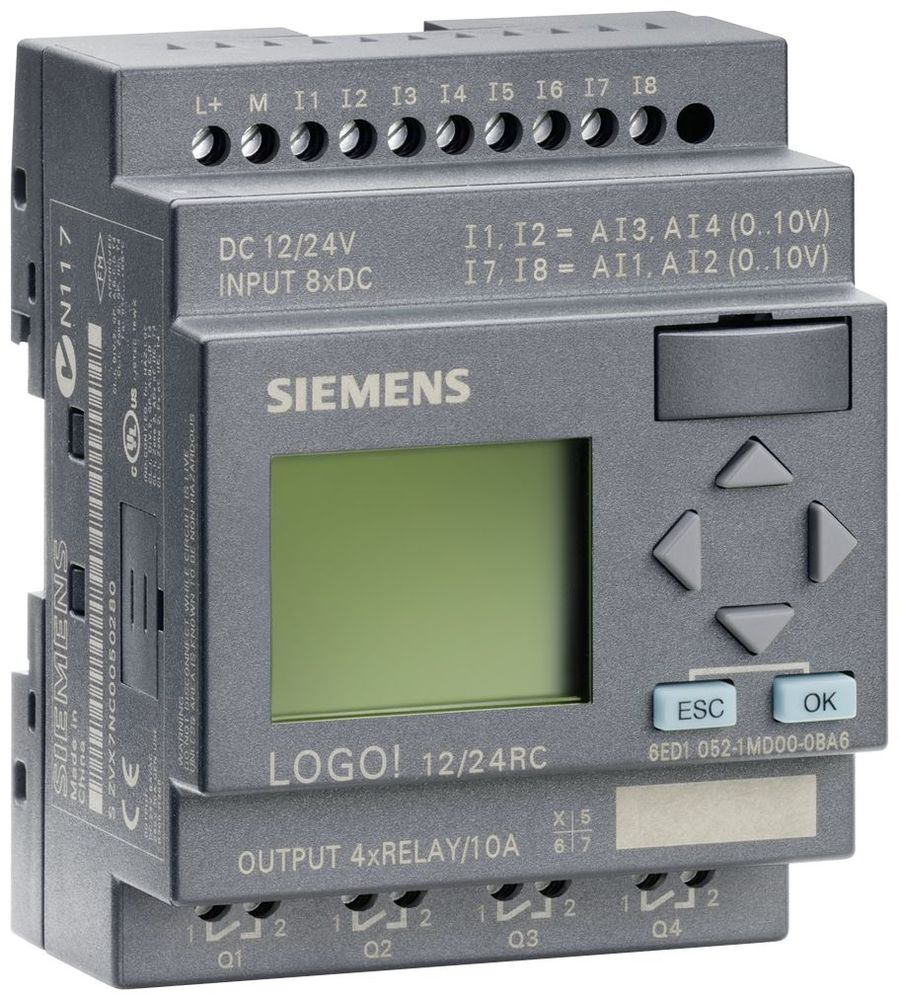
\includegraphics[width=10cm]{plc}
\end{center}
\subsection*{Construction}
PLCs have a power supply for internal logic controls and the opening and closing of its coils. They typically have several digital (boolean) inputs, and a handful of analogue (variable voltage or variable current input, depending on its designated configuration). Some PLCs can be directly programmed from the unit itself -- though, this is considered a high end feature. Rather, the program to be run on the device is usually uploaded by cable, SD card or USB flash drive and initially created on a Microsoft Windows computer, using the specialized software created by the PLC's manufacturer.
\subsection*{Operation}
Simplified operation of the PLC is as follows: Input, output. That is to say, an input signal is received -- either by a digital or analogue (arithmetic-triggered) input, or by the PLC's internal logic, such as internal clock or timer -- and an output signal is sent. This can be either to another PLC, or more commonly to a contactor coil, with the intention of closing the contactor -- energizing a piece of machinery, such as an induction motor.
\section{Thermal Overload Relays}
Thermal Overload Relays, or Thermal Protection Units (TPUs) are devices placed in series with the primary AC phases ($\Phi$) being supplied to a consumer, typically an induction motor.
\begin{center}
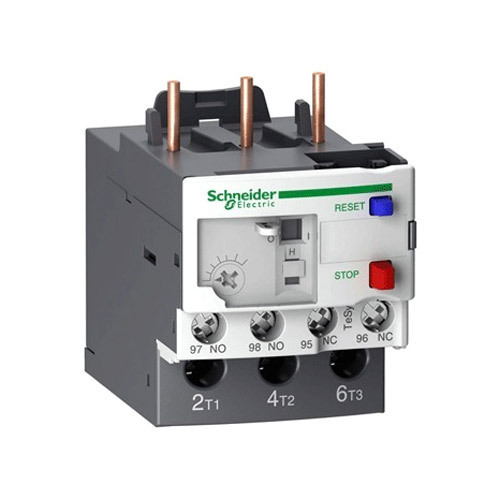
\includegraphics[width=10cm]{thermal}
\end{center}
\subsection*{Construction}
TPUs typically have three terminals in, three terminals out for the three phase AC, as well as an adjustable current setting range, a status indicator, a reset button, and often have signaling contacts for PLC use. Inside the TPU is a bimetallic strip, one for each phase, which as well as a circuit breaker surrounded by a moulded plastic case.
\subsection*{Operation}
Due to mechanical overloading a consumer may draw excessive currents, the heat generated by which may cause the bimetallic strip inside the TPU to bend, closing a contact, which causes all three phases to trip open. This device must be reset manually before operation resumes. The dial on the front of the TPU can be adjusted to change the current which will trip the circuit breaker. This is done by physically moving the contact which needs to be closed by the bimetallic strip.
% BEGINNING OF LEARNING OUTCOME 2
\section{Learning Outcome 2}
\begin{tcolorbox}[colback=red!5!white,colframe=red!75!black,title=\textbf{Demonstrating the use of appropriate test equipment and accurately interpret results }]
This outcome is covered by a written report:-

Examine the condition of a typical Three phase squirrel cage induction motor is evaluated using measuring instruments, use photos to support your findings.
\end{tcolorbox}
\newpage
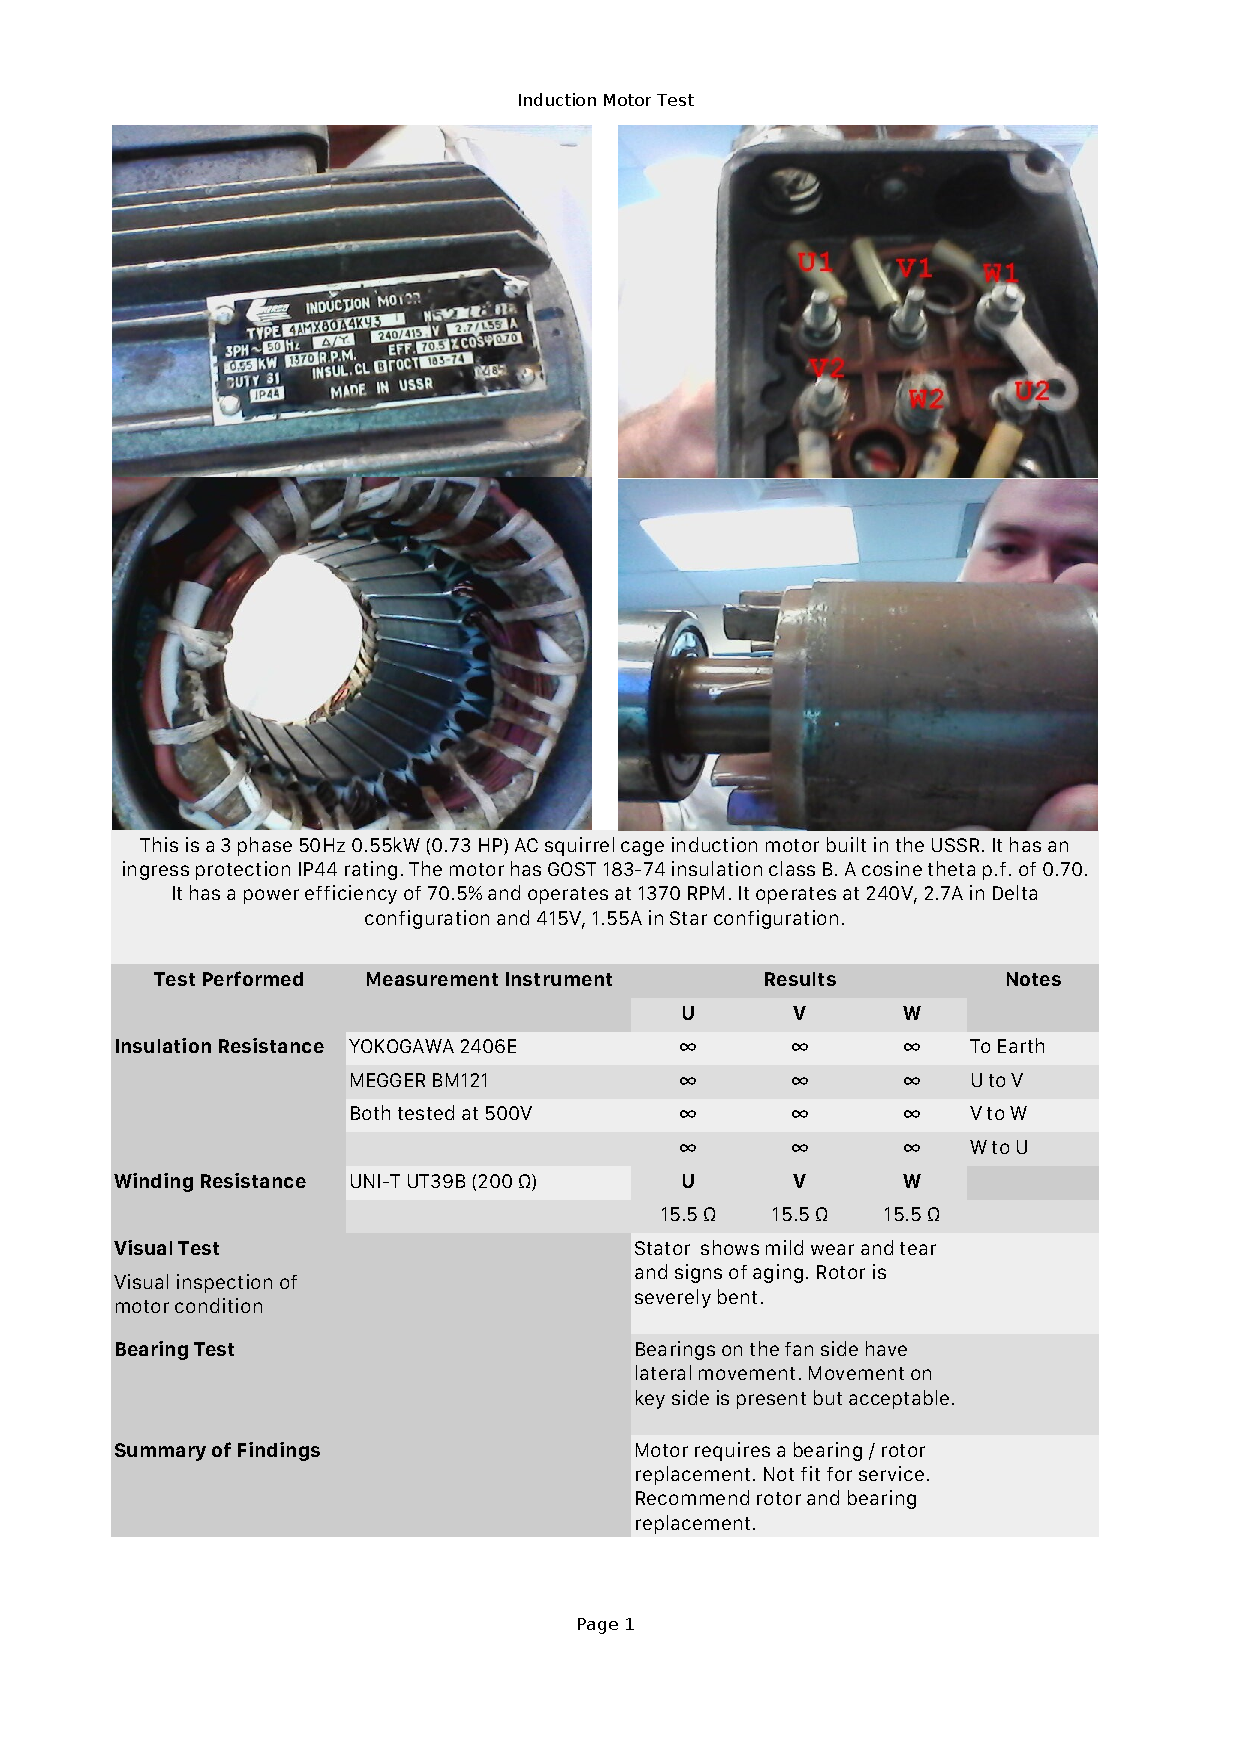
\includepdf[pages={1}]{2.pdf}
\newpage
% BEGINNING OF LEARNING OUTCOME 3
\section{Learning Outcome 3}
\begin{tcolorbox}[colback=red!5!white,colframe=red!75!black,title=\textbf{Demonstrate basic knowledge of procedures for the conduct of repair and maintenance in accordance with manuals and good practice}]
This section is covered through practice tasks in the Marine Worksop at Mahurangi campus, it also takes into account the machine-shop exercises completed at MIT south campus in March.

Demonstrating a basic understanding for use of machine tools, hand tools and power tools
\end{tcolorbox}
\end{document}
